\documentclass[a4paper,12pt]{article}

% Load amsmath first
\usepackage{amsmath}

\usepackage{amssymb}
\usepackage{amsthm} % Add this line for theorems and lemmas

\usepackage{tikz}
\usepackage{pgfplots}

\usepackage{breqn} 
\newcommand{\circled}[1]{\tikz[baseline=(char.base)]{
            \node[shape=circle,draw,inner sep=2pt] (char) {#1};}}

\usepackage{graphicx}
\usepackage{float}
\usepackage{multicol}
\usepackage{geometry}
\geometry{a4paper, margin=1in}
\usepackage{hyperref}
\hypersetup{
    colorlinks=true,
    linkcolor=blue,
    filecolor=blue,
    urlcolor=blue,
    pdftitle={Overleaf Example},
    pdfpagemode=FullScreen,
}
% Load fancyhdr for custom headers
\usepackage{fancyhdr}
\pagestyle{fancy}
% Then load polyglossia and bidi
\usepackage{polyglossia}
\usepackage{bidi}

% Set languages and fonts
\setdefaultlanguage{hebrew}
\setotherlanguage{english}
\newfontfamily\hebrewfont[Script=Hebrew]{David CLM}
\newfontfamily\hebrewfonttt[Script=Hebrew]{Miriam Mono CLM} % For monospace
\setmainfont{David CLM}
\setlength{\parindent}{0pt}

\title{שיטות לעיבוד תמונה: GrabCut ו-Poisson Blending}
\author{אור פחימה}
\date{07/07/2024}

\begin{document}

\maketitle

\section*{מבוא}

בעבודה זו נעסוק בשני אלגוריתמים חשובים בתחום עיבוד התמונה: GrabCut ו-Poisson Blending. 
אלגוריתם GrabCut משמש לחיתוך רקע מתמונה ומבוסס על שילוב של מודלים סטטיסטיים והצגת גרפים. 
לעומתו, אלגוריתם Poisson Blending מאפשר שילוב חלק של אובייקטים מתוך תמונות שונות על ידי פתרון משוואות דיפרנציאליות חלקיות, וכך יוצר תוצאות טבעיות ומציאותיות יותר.
\subsection*{GrabCut}

מימשתי את האלגוריתם על פי האמור במאמר (עם קצת תוספות):

\begin{enumerate}
    \item \textbf{אתחול המודלים}: כפי שמופיע במאמר, חישבתי את המרכזים בעזרת KMeans כדי לאפשר אתחול מהיר ומדויק ככל הניתן. בניתי את המודלים עבור הרקע והקדמה, ואתחלתי את המשקלים והשונויות של כל אחד מהרכיבי המודלים.
    \item \textbf{עדכון המודלים}: בשלב זה, כפי שצויין במאמר, אין צורך באתחול מחדש של המרכזים, אלא נשתמש במודלים הישנים על מנת לאתחל מרכזים חדשים לבניית מודלים חדשים עם שוניות אחרות ומשקלים שונים.
    \item \textbf{חישוב החתך המינימלי}: עבור שיטה זו השתמשתי באלגוריתם min cut של החבילה \texttt{igraph}. בניית הגרף וכל מה שקשור בו מבוצעים בקובץ אחר בשם \texttt{utils}.
        \begin{enumerate}
            \item \textbf{הליך בניית הגרף וחישוב בטא וקשתות מסוג N ו-T}: מבוצעים על פי הנוסחאות המתמטיות המוזכרות במאמר, כאשר על מנת לייעל את הריצה, קשתות מסוג N נשמרות על מנת לחשב פעם אחת בלבד בכל ריצת האלגוריתם.
        \end{enumerate}
    \item \textbf{עדכון המסיכה}: מתבצע בעזרת החתך שנמצא בריצה.
    \item \textbf{התכנסות} : 
    האלגוריתם עוצר את ריצתו עבור כל אחד מהתנאים הבאים :\\ 
    - אם האנרגיה בגרף לא התשתנה מעל לנקודת סף .\\ 
    - אם אף אחד מהפיקסלים לא השתנה באיטרציה . 
    אני מבין שהתנאים אמורים להיות שקולים , אך ראיתי לנכון הואיל והאלגוריתם הסתברותי בסופו של דבר ומתצפיות שכאשר לא משתנים פיקסלים אין למה להמשיך את הריצה. 
\end{enumerate}

\subsection*{שינויים ושיפורים שביצעתי}

\begin{itemize}
    \item מצאתי שיעיל להעביר את התמונה בפילטר מדיאן, שהוא מבצע טשטוש אך עדיין שומר על הקצוות.
    \item בנוסף, מאחר והאלגוריתם מבצע המון חישובים ורץ על הרבה מידע, על מנת לייעל ולהקטין את זמן הריצה, הקטנתי את התמונה בחצי בתחילת הריצה.
\end{itemize}

\section*{תוצאות הריצה}

להלן התוצאות שהתקבלו מהרצת האלגוריתם על כל התמונות בתיקייה \texttt{data} תוך שימוש במלבנים המוכנים:

\begin{figure}[H]
    \centering
    \begin{minipage}{0.3\textwidth}
        \centering
        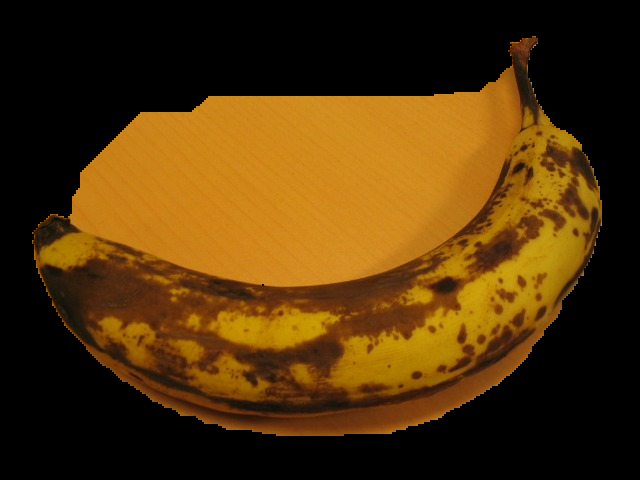
\includegraphics[width=\textwidth]{my_reasults/final_img/banana1_result.png}
        \caption{תוצאה עבור תמונת banana1}
    \end{minipage}
    \hfill
    \begin{minipage}{0.3\textwidth}
        \centering
        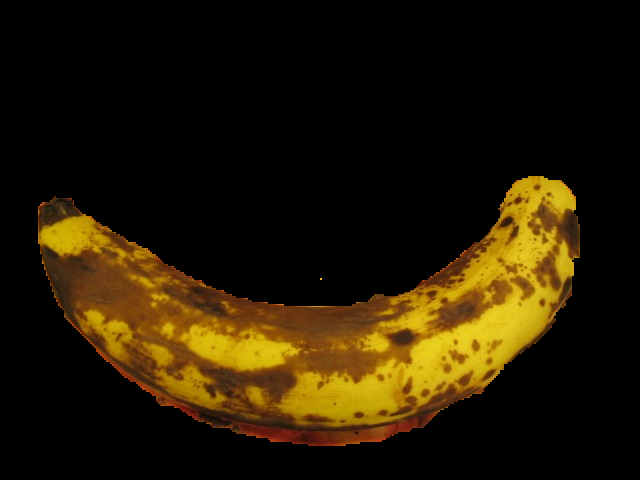
\includegraphics[width=\textwidth]{my_reasults/final_img/banana2_result.png}
        \caption{תוצאה עבור תמונת banana2}
    \end{minipage}
    \hfill
    \begin{minipage}{0.3\textwidth}
        \centering
        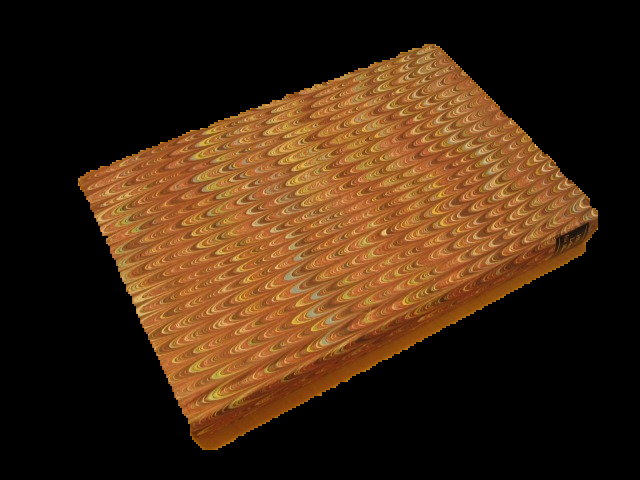
\includegraphics[width=\textwidth]{my_reasults/final_img/book_result.png}
        \caption{תוצאה עבור תמונת book}
    \end{minipage}
\end{figure}

\begin{figure}[H]
    \centering
    \begin{minipage}{0.3\textwidth}
        \centering
        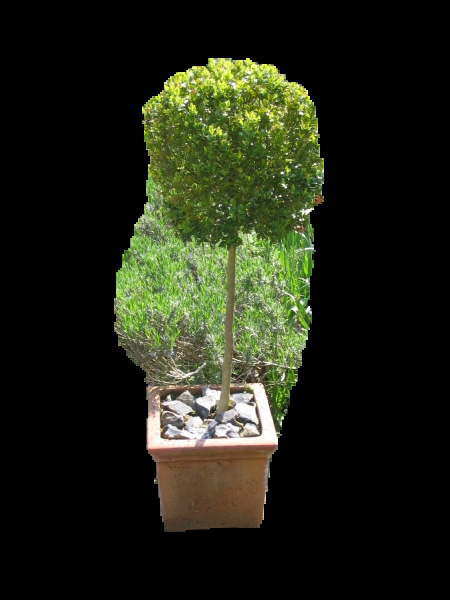
\includegraphics[width=\textwidth]{my_reasults/final_img/bush_result.png}
        \caption{תוצאה עבור תמונת bush}
    \end{minipage}
    \hfill
    \begin{minipage}{0.3\textwidth}
        \centering
        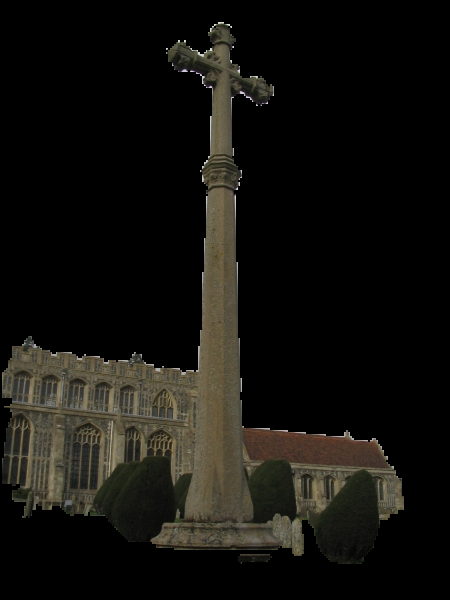
\includegraphics[width=\textwidth]{my_reasults/final_img/cross_result.png}
        \caption{תוצאה עבור תמונת cross}
    \end{minipage}
    \hfill
    \begin{minipage}{0.3\textwidth}
        \centering
        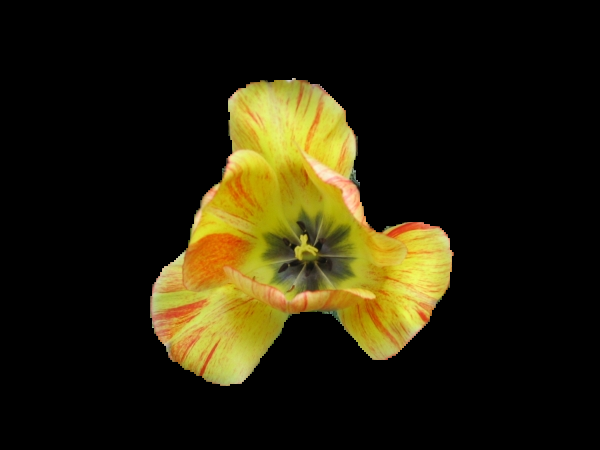
\includegraphics[width=\textwidth]{my_reasults/final_img/flower_result.png}
        \caption{תוצאה עבור תמונת flower}
    \end{minipage}
\end{figure}

\begin{figure}[H]
    \centering
    \begin{minipage}{0.3\textwidth}
        \centering
        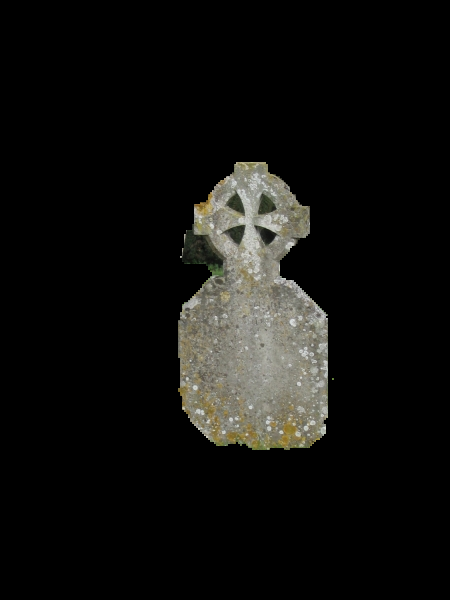
\includegraphics[width=\textwidth]{my_reasults/final_img/grave_result.png}
        \caption{תוצאה עבור תמונת grave}
    \end{minipage}
    \hfill
    \begin{minipage}{0.3\textwidth}
        \centering
        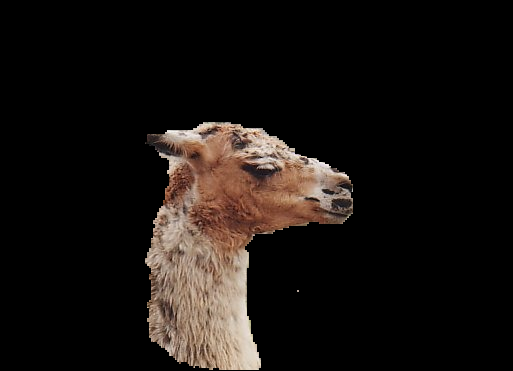
\includegraphics[width=\textwidth]{my_reasults/final_img/llama_result.png}
        \caption{תוצאה עבור תמונת llama}
    \end{minipage}
    \hfill
    \begin{minipage}{0.3\textwidth}
        \centering
        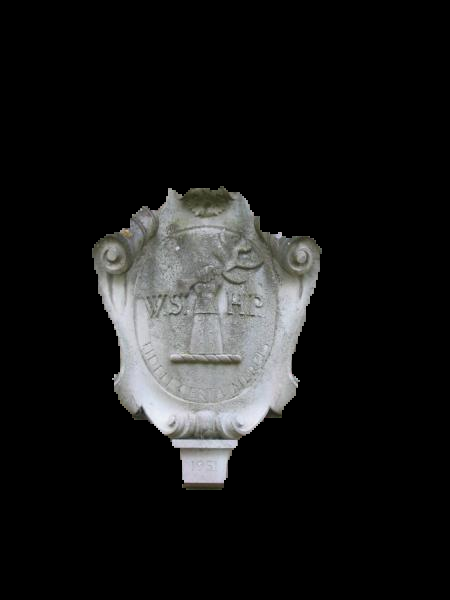
\includegraphics[width=\textwidth]{my_reasults/final_img/memorial_result.png}
        \caption{תוצאה עבור תמונת memorial}
    \end{minipage}
\end{figure}

\begin{figure}[H]
    \centering
    \begin{minipage}{0.3\textwidth}
        \centering
        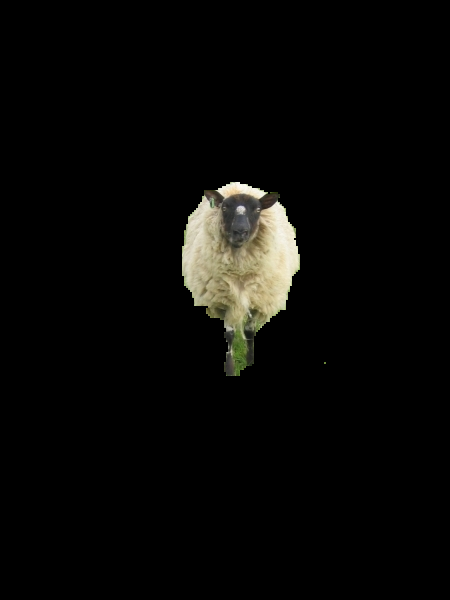
\includegraphics[width=\textwidth]{my_reasults/final_img/sheep_result.png}
        \caption{תוצאה עבור תמונת sheep}
    \end{minipage}
    \hfill
    \begin{minipage}{0.3\textwidth}
        \centering
        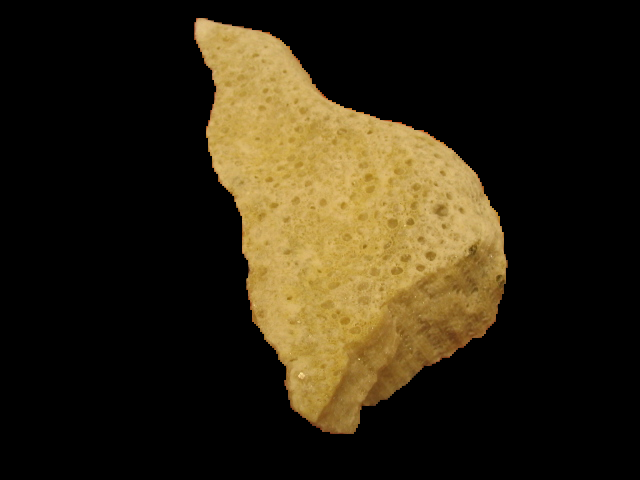
\includegraphics[width=\textwidth]{my_reasults/final_img/stone2_result.png}
        \caption{תוצאה עבור תמונת stone2}
    \end{minipage}
    \hfill
    \begin{minipage}{0.3\textwidth}
        \centering
        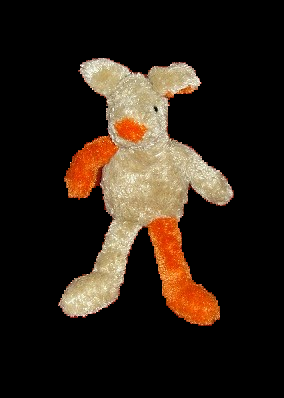
\includegraphics[width=\textwidth]{my_reasults/final_img/teddy_result.png}
        \caption{תוצאה עבור תמונת teddy}
    \end{minipage}
\end{figure}

\subsection*{מדדים}

\begin{table}[H]
\centering
\begin{tabular}{|c|c|c|}
\hline
\textbf{Img name} & \textbf{Accuracy} & \textbf{Jaccard} \\
\hline\hline
banana1 & 74.7705078125 & 50.36789426161796 \\
\hline
banana2 & 97.56282552083333 & 90.31536192890775 \\
\hline
book & 97.72688802083334 & 94.18950066151325 \\
\hline
bush & 88.47703703703704 & 58.54662705021785 \\
\hline
cross & 88.15037037037037 & 68.31806703965935 \\
\hline
flower & 99.48185185185186 & 97.38406881077039 \\
\hline
grave & 98.6237037037037 & 89.31600586527126 \\
\hline
llama & 98.13212275972951 & 89.45260347129505 \\
\hline
memorial & 97.66703703703705 & 87.56269004462347 \\
\hline
sheep & 99.53925925925927 & 91.68393609198476 \\
\hline
stone2 & 99.54361979166667 & 98.1457233927178 \\
\hline
teddy & 99.24357704013022 & 96.49977483931715 \\
\hline
\end{tabular}
\caption{Results table}
\label{tab:results}
\end{table}

\newpage
\section*{ניתוח הייפר פרמטרים ותוצאה של טשטוש}

\subsection*{השפעת שינוי פרמטר גמא}

פרמטר גמא בעצם המכפיל כל קשת מסוג N שולט לנו בעצם על כמה אנחנו ממשקלים דמיון בין פיקסלים שכנים בריצה. כלומר ככל שיגדל האלגוריתם יעדיף להשאיר יותר פיקסלים דומים אחד ליד השני.
\subsubsection*{עבור גמא = 10
}

\begin{figure}[H]
\centering
\begin{tabular}{ccc}
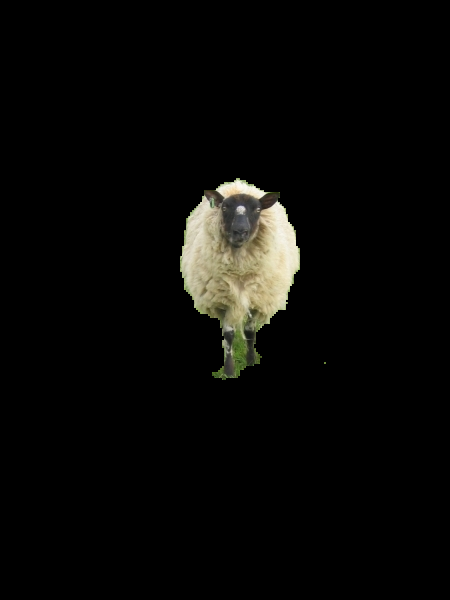
\includegraphics[width=0.3\textwidth]{my_reasults/gamma10/sheep_result.png} &
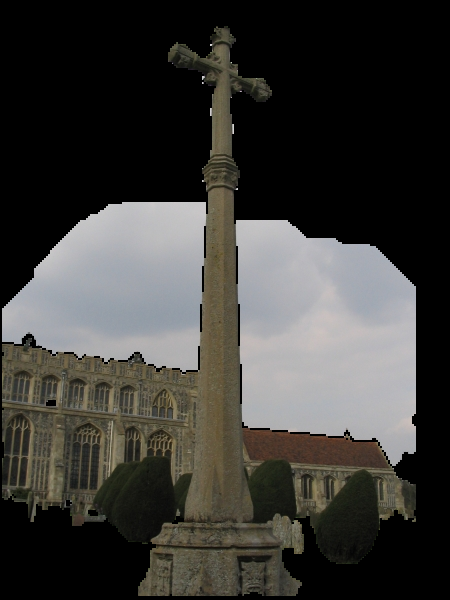
\includegraphics[width=0.3\textwidth]{my_reasults/gamma10/cross_result.png} \\
\end{tabular}
\caption{תוצאות עבור גמא = 10}
\end{figure}

ניתן לראות שכאשר אנו מורידים את ערכו אנו מתעדפים פחות דמיון בצבעים מה שגורם לירידה בביצועים על התמונה של הצלב, למרות שלהפתעתי יש לומר בתמונה של הכבשה מתקבלת תוצאה טיפה יותר טובה.

\subsubsection*{עבור גמא = 200
}

\begin{figure}[H]
\centering
\begin{tabular}{ccc}
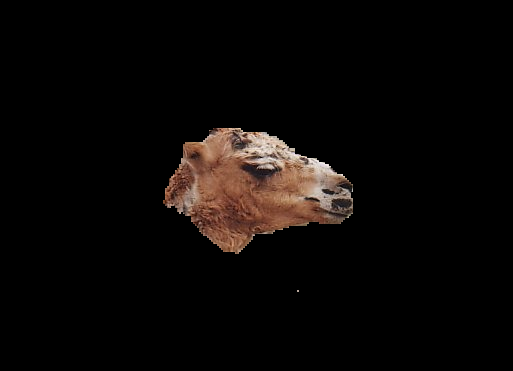
\includegraphics[width=0.3\textwidth]{my_reasults/gamma200/llama_result.png} &
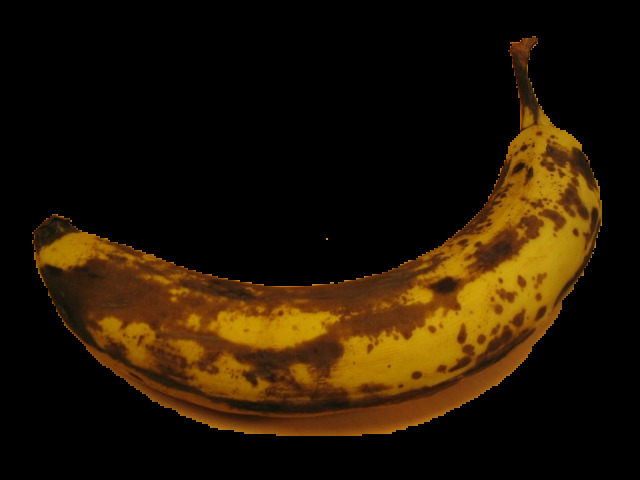
\includegraphics[width=0.3\textwidth]{my_reasults/gamma200/banana1_result.png} \\
\end{tabular}
\caption{תוצאות עבור גמא = 200}
\end{figure}

על אותו ההגיון כאשר גמא מאוד גדול האלגוריתם פחות מעדיף להפריד פיקסלים דומים ורואים את ההשפעתו בתמונה של הלמה, למרות שאני חייב לציין שעבור התמונה של בננה 1 בשום שינוי של פרמטר לא הצלחתי להגיע לתוצאה טובה כמו זו.


\subsection{כמות הגאוסיאנים}
בדקתי את המודל עבור 2 ו-10 גאוסיאנים. אציין שלא ראיתי שינויים דרסטיים ששווה לציין. אינטואיטיבית ברור לי שככל שיהיו פחות גאוסיאנים אני עלול להגיע לתוצאה של "חוסר התאמה" למול מצב שבו יש יותר מדי גאוסיאנים ועלולים להגיע למצב של "התאמת יתר".

\begin{figure}[H]
    \centering
    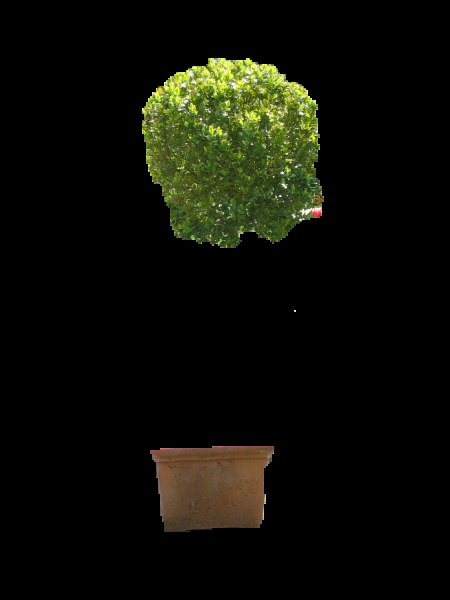
\includegraphics[width=0.3\textwidth]{my_reasults/comp2/bush_result.png}
    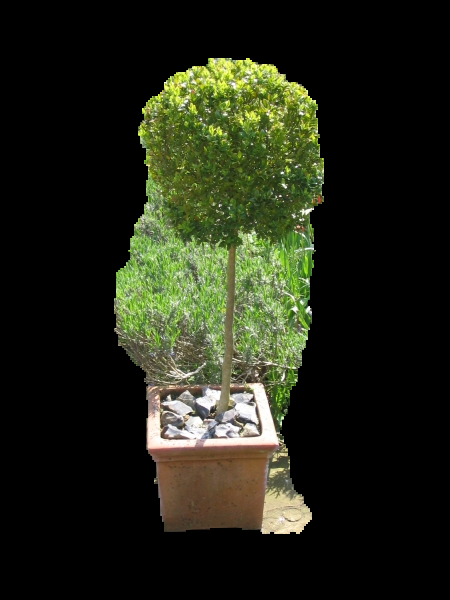
\includegraphics[width=0.3\textwidth]{my_reasults/comp10/bush_result.png}
    \caption{השוואת כמות גאוסיאנים - 2 גאוסיאנים (שמאל) ו-10 גאוסיאנים (ימין)}
\end{figure}
\subsection{השפעת טשטוש}
כמו שציינתי בפסקת המימוש, אני השתמשתי בפילטר מדיאן שהביא לי תוצאות טובות. האמת שגם פילטר הגאוסיאן שמשמש לטשטוש עוזר להגיע לתוצאות טובות בתמונות מסוימות.

\subsubsection{טשטוש קטן}
השתמשתי בקרנל של 5x5.
\begin{figure}[H]
    \centering
    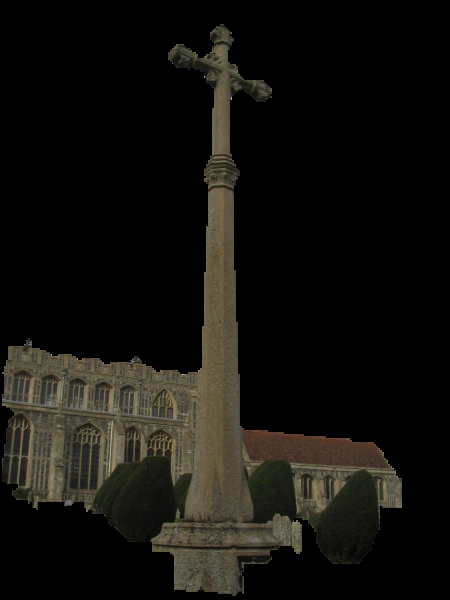
\includegraphics[width=0.3\textwidth]{my_reasults/smallblur/cross_result.png}
    \caption{תוצאה עבור טשטוש קטן - קרנל 5x5}
\end{figure}
ניתן לראות שהשימוש בפילטר זה (במידה נכונה) אכן נותן תוצאה טובה יותר עבור התמונה של הצלב.

\subsubsection{טשטוש גדול}
השתמש בקרנל של 21x21. אינטואיטיבית ברור שטשטוש במידה לא נכונה עלול לטשטש עבורנו את הקצוות של האובייקט ובכך ליצור סגמנטציה שהיא פחות טובה.
\begin{figure}[H]
    \centering
    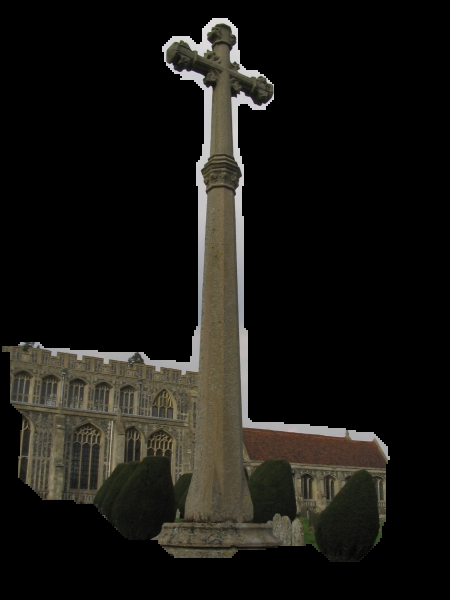
\includegraphics[width=0.3\textwidth]{my_reasults/highblur/cross_result.png}
    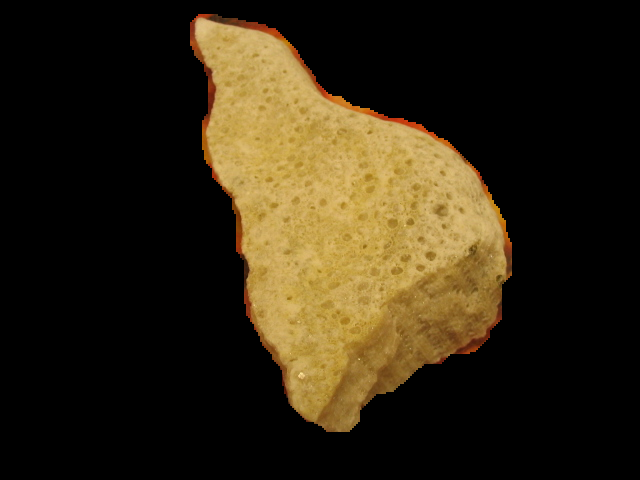
\includegraphics[width=0.3\textwidth]{my_reasults/highblur/stone2_result.png}
    \caption{תוצאה עבור טשטוש גדול - קרנל 21x21}
\end{figure}
\subsection{זמני ריצה}
לאחר הקטנת התמונה בחצי, זמני הריצה הממוצעים הם 8 - 30 שניות, בתלות בפיזור הצבעים בתמונה, גודל המסיכה, כמות הפיקסלים. האלגוריתם מתכנס לרוב לאחר 5 - 12 איטרציות.

כמו כן, ניתן לראות את התנהגות האנרגיה עבור ריצות נבחרות:
\begin{figure}[H]
    \centering
    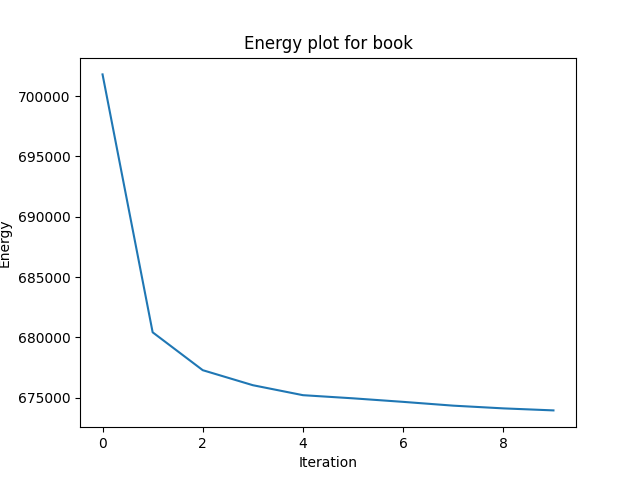
\includegraphics[width=0.3\textwidth]{my_reasults/book_energy.png}
    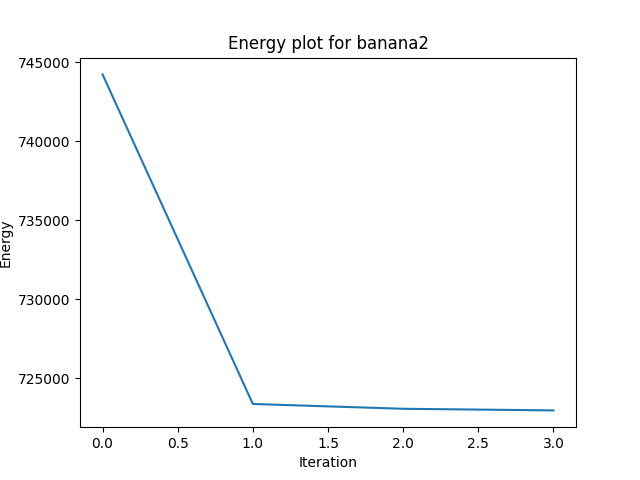
\includegraphics[width=0.3\textwidth]{my_reasults/banana2_energy.png}
    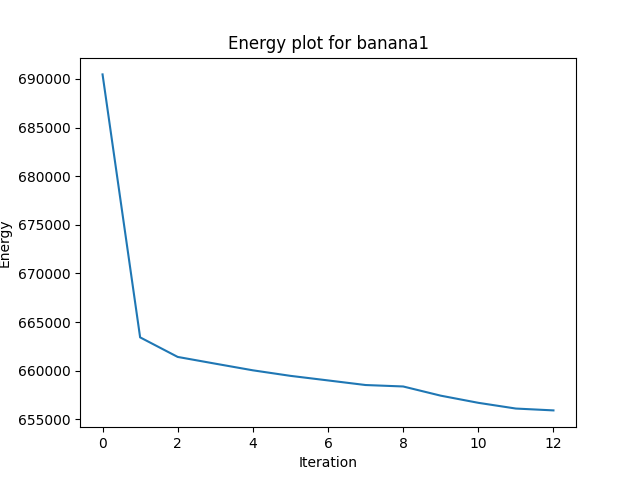
\includegraphics[width=0.3\textwidth]{my_reasults/banana1_energy.png}
    \caption{התנהגות האנרגיה עבור ריצות נבחרות}
\end{figure}
\pagebreak
\subsection{מגבלות המימוש וקשיים}
כפי שניתן לראות מהתוצאות בריצות, כאשר הצבעים של האובייקט אותו רוצים לחתוך דומה מאוד לצבעי הרקע שלו, לאלגוריתם קשה מאוד לסגמנט את האובייקט (עד כדי חוסר הצלחה ברוב המקרים). ניתן לראות זאת היטב בתמונות של בננה1 והעציץ:
\begin{figure}[H]
    \centering
    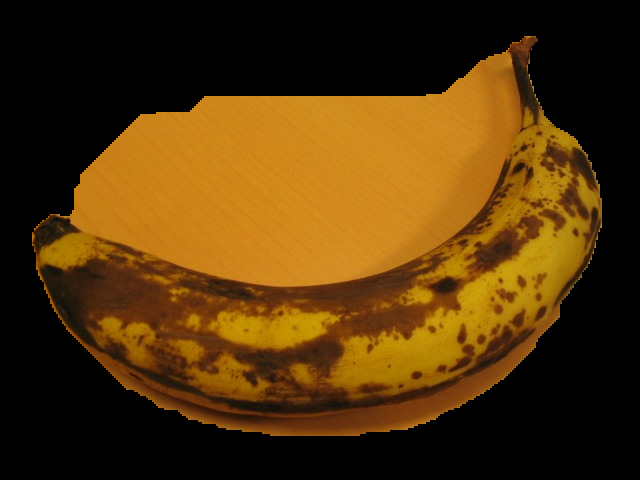
\includegraphics[width=0.3\textwidth]{{my_reasults/final_img/banana1_result.png}}
    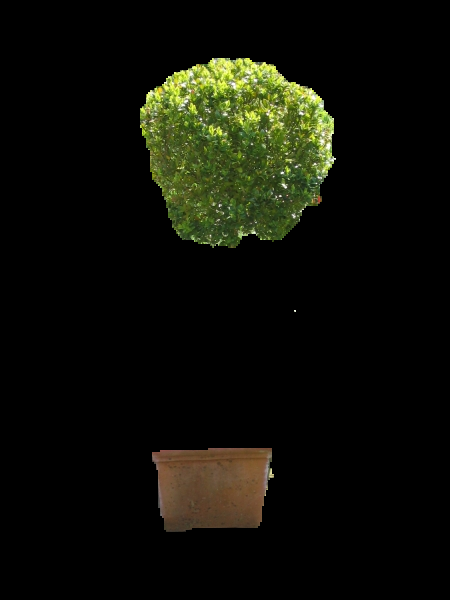
\includegraphics[width=0.3\textwidth]{{my_reasults/final_img/bush_result.png}}
    \caption{תוצאות ריצה עבור בננה1 והעציץ}
\end{figure}

בנוסף, גילוי נאות: הקטנתי את המסיכה המוכנה של התמונה של הצלב. זוהי עוד אחת ממגבלות הריצה כאשר אין מספיק פיקסלי רקע לאלגוריתם להתבסס עליהם, הוא לא מצליח בכלל לזהות את האובייקט. ניתן לראות את התוצאה לפי שינוי ערכי המלבן:
\begin{figure}[H]
    \centering
    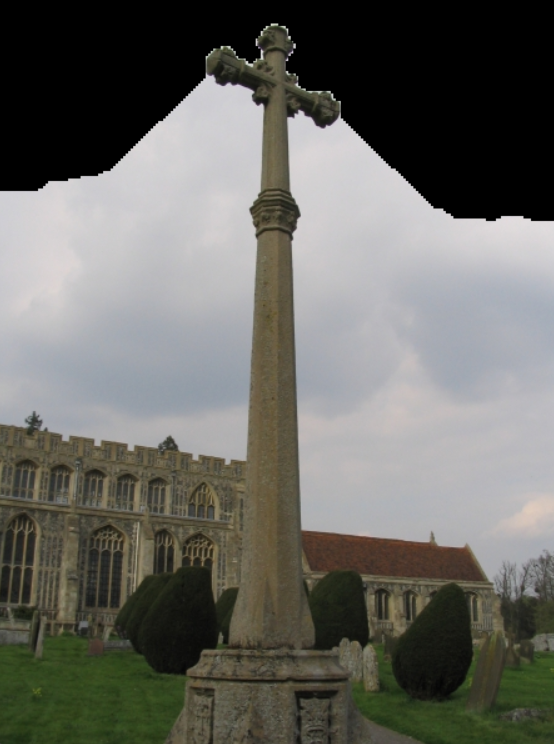
\includegraphics[width=0.3\textwidth]{my_reasults/cross.png}
    \caption{תוצאות ריצה עבור הצלב עם מסיכה מוקטנת}
\end{figure}
\newpage
\section{מימוש Poisson Blending}


תחילה, האלגוריתם ממיר את תמונות המקור והיעד לפורמט \texttt{float32} כדי למנוע גלישת ערכים במהלך החישוב. לאחר מכן, הוא מזהה את האינדקסים של הפיקסלים במסכה ומחשב את אופרטור הלפלסיאן. אופרטור הלפלסיאן משמש לחישוב ההבדלים בין פיקסלים שכנים בתמונה.

האלגוריתם יוצר מטריצת דלילה \texttt{A} ומטריצת \texttt{b} שמייצגות את מערכת המשוואות הלינאריות שיש לפתור. מטריצת \texttt{A} כוללת את המשקלים של קשתות מסוג N וחיבור הפיקסלים במסכה לפיקסלים הסובבים בתמונה המקורית, בעוד מטריצת \texttt{b} כוללת את התרומות של הערכים מתמונת היעד ומהתמונה המקורית.

לאחר מכן, האלגוריתם פותר את מערכת המשוואות עבור כל ערוץ צבע בנפרד ומשלב את התוצאה באזור המסכה בתמונת היעד. התוצאה הסופית נשמרת כתמונת uint8 לאחר עדכון הערכים לטווח התקני 
[0, 255].
\subsection*{השפעת מסיכה לא הדוקה}

בעמוד הבא מוצגות תוצאות הריצה עבור כל המסיכות שהתקבלו. ניתן לראות שגם כאשר המסיכה שהתקבלה לא הייתה מדויקת, כמו בתמונות של בננה1 והעציץ, האלגוריתם מצליח להתמודד עם הקושי ולהניב תוצאות טובות.

\newpage
\section{תוצאות הריצה}

\begin{figure}[H]
    \centering
    \begin{tabular}{ccc}
        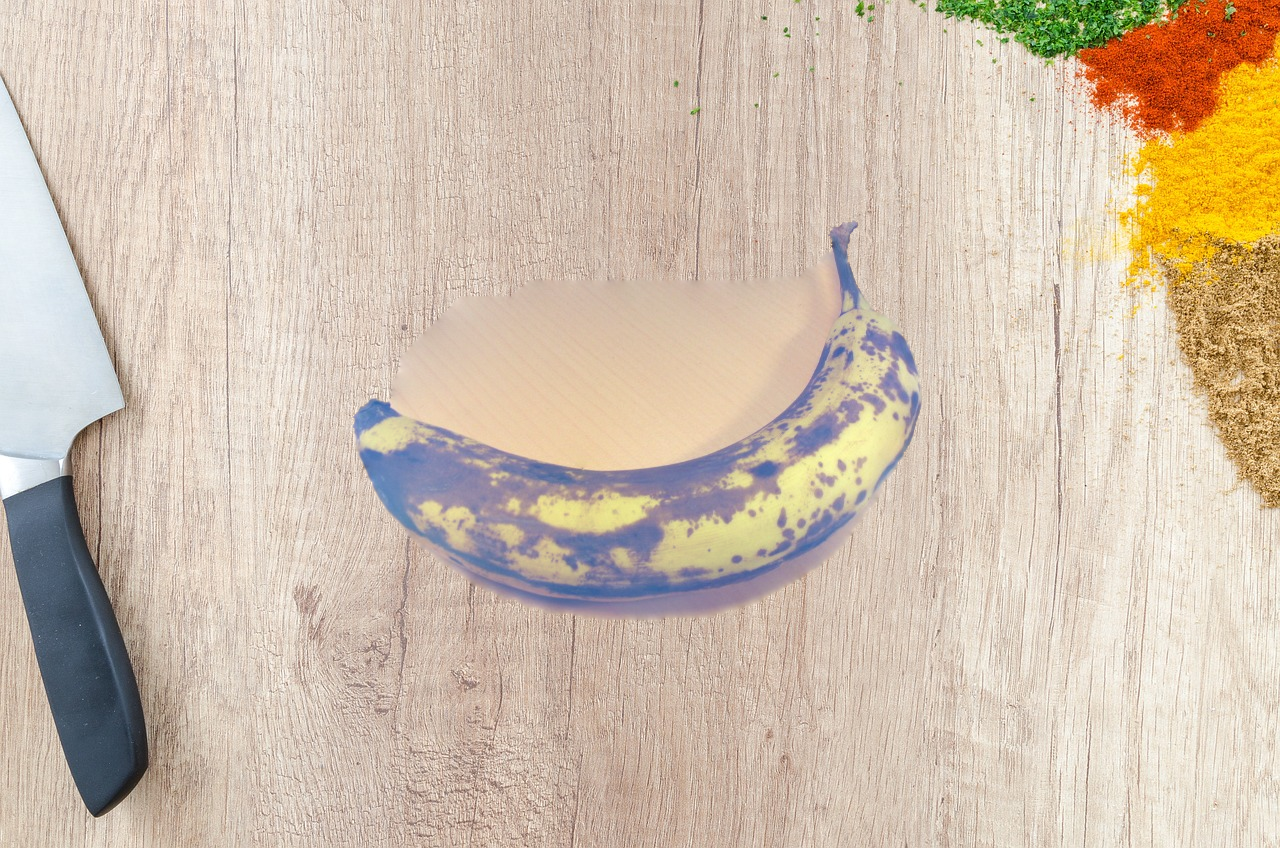
\includegraphics[width=0.3\textwidth]{my_reasults/PS_res/banan1_result.png} & 
        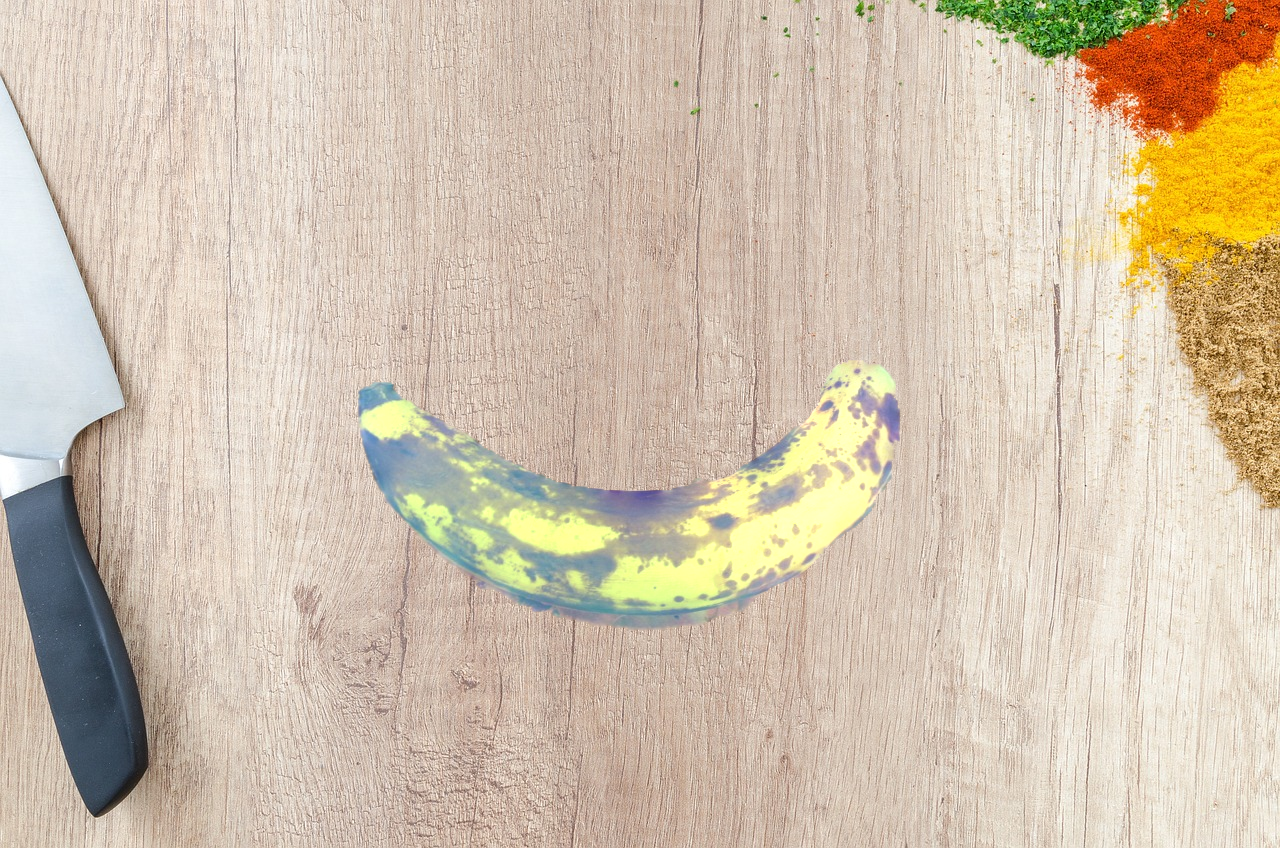
\includegraphics[width=0.3\textwidth]{my_reasults/PS_res/banana2_result.png} & 
        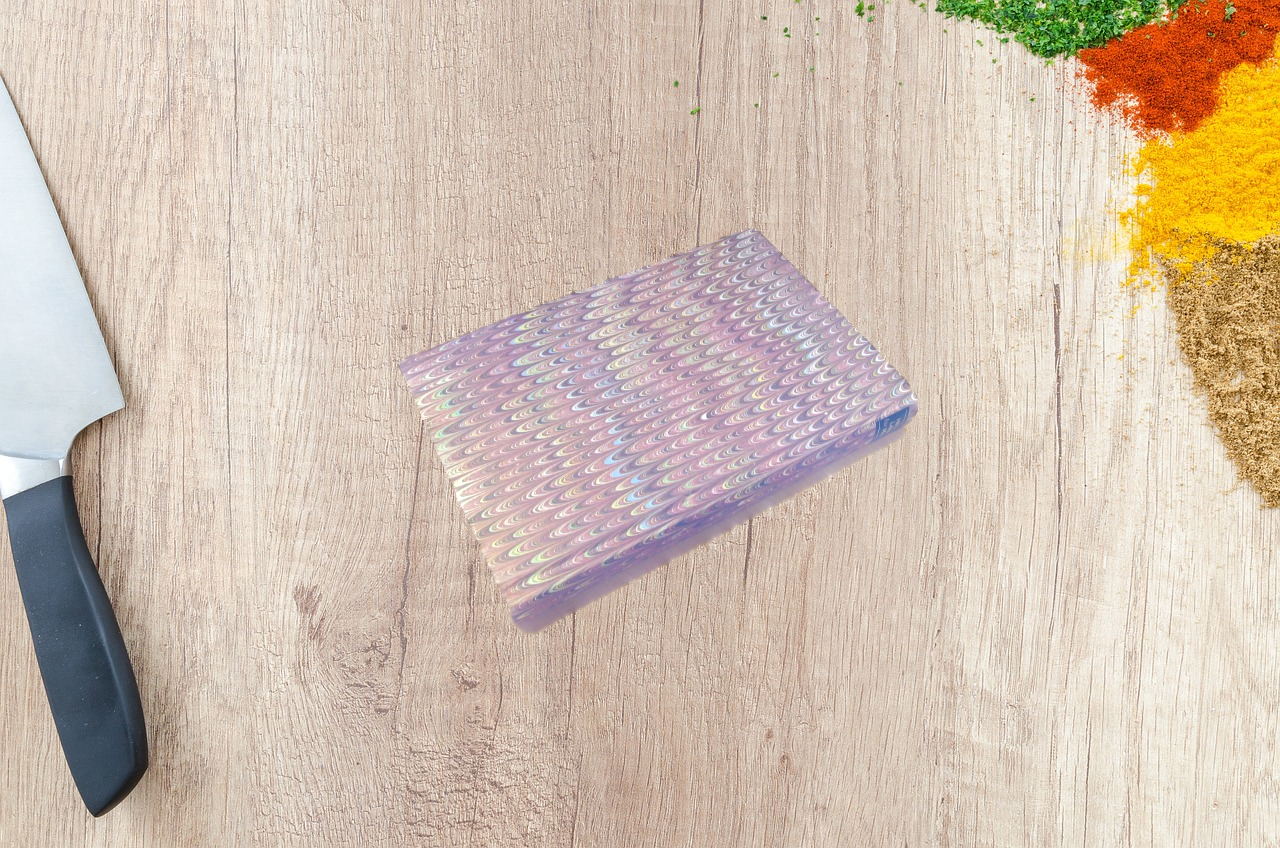
\includegraphics[width=0.3\textwidth]{my_reasults/PS_res/book_result.png} \\
        \textbf{Banana 1} & \textbf{Banana 2} & \textbf{Book} \\
        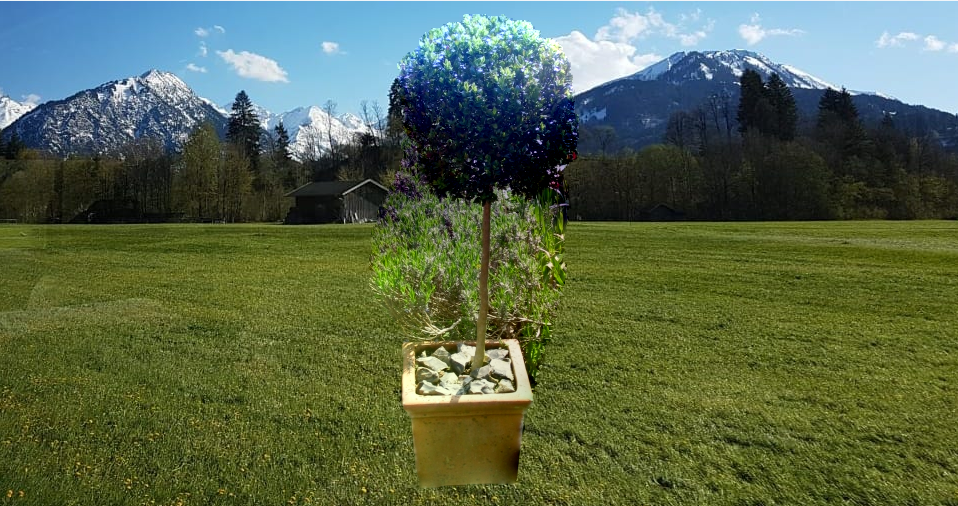
\includegraphics[width=0.3\textwidth]{my_reasults/PS_res/bush_result.png} & 
        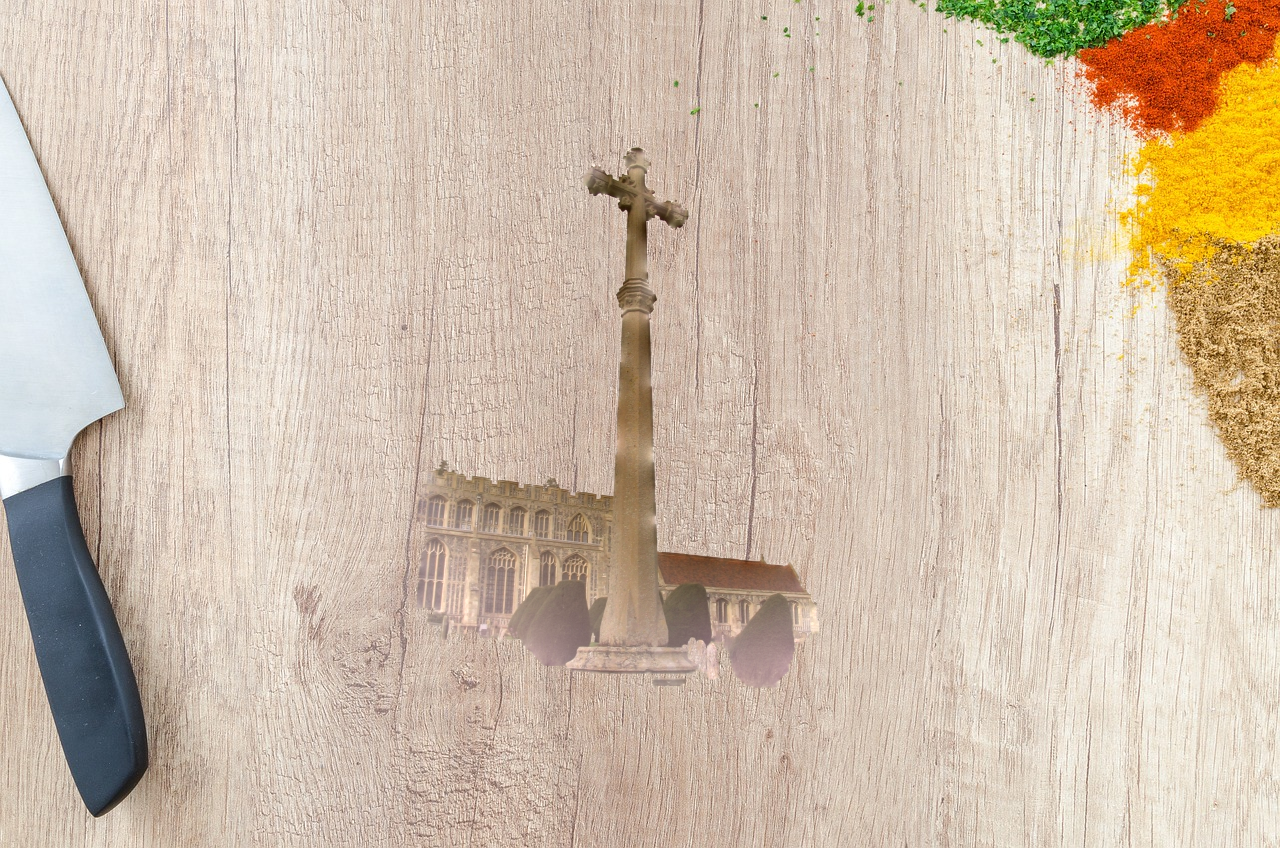
\includegraphics[width=0.3\textwidth]{my_reasults/PS_res/cross_result.png} & 
        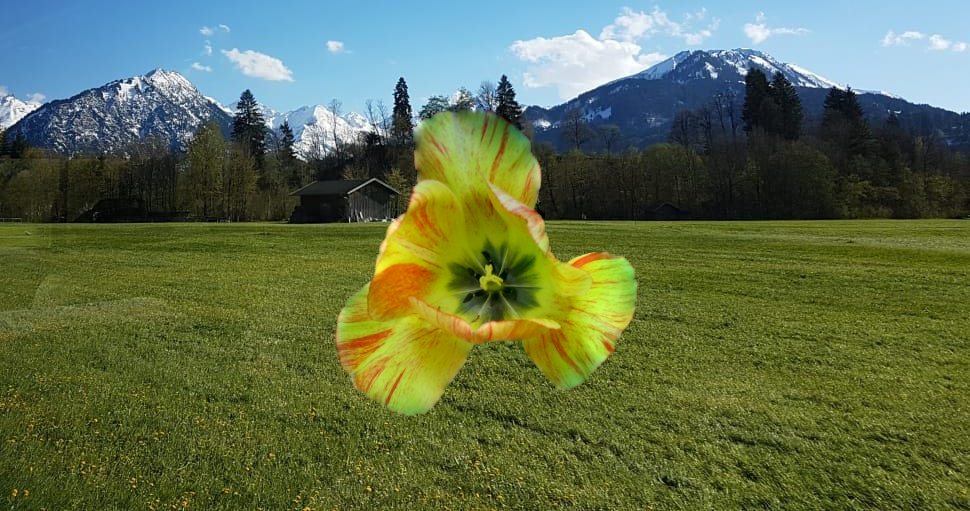
\includegraphics[width=0.3\textwidth]{my_reasults/PS_res/flower_result.png} \\
        \textbf{Bush} & \textbf{Cross} & \textbf{Flower} \\
        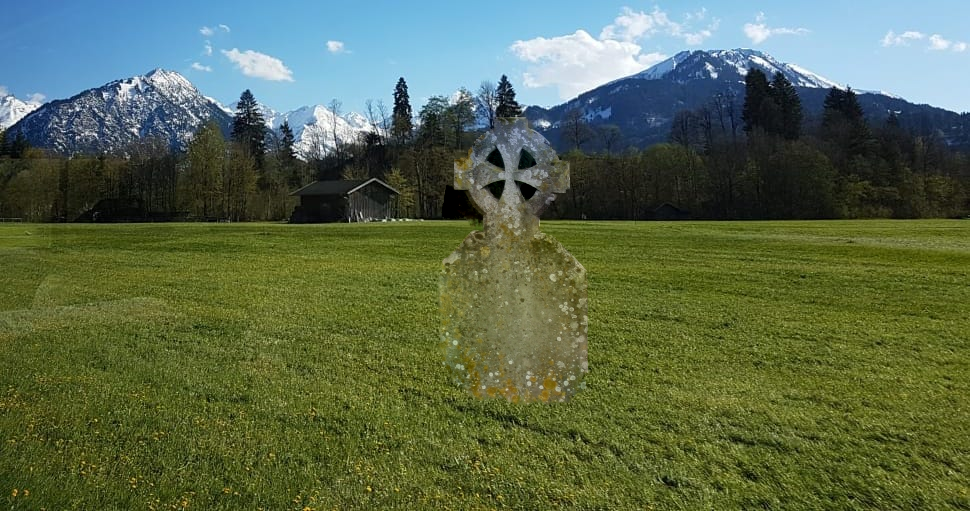
\includegraphics[width=0.3\textwidth]{my_reasults/PS_res/grave_result.png} & 
        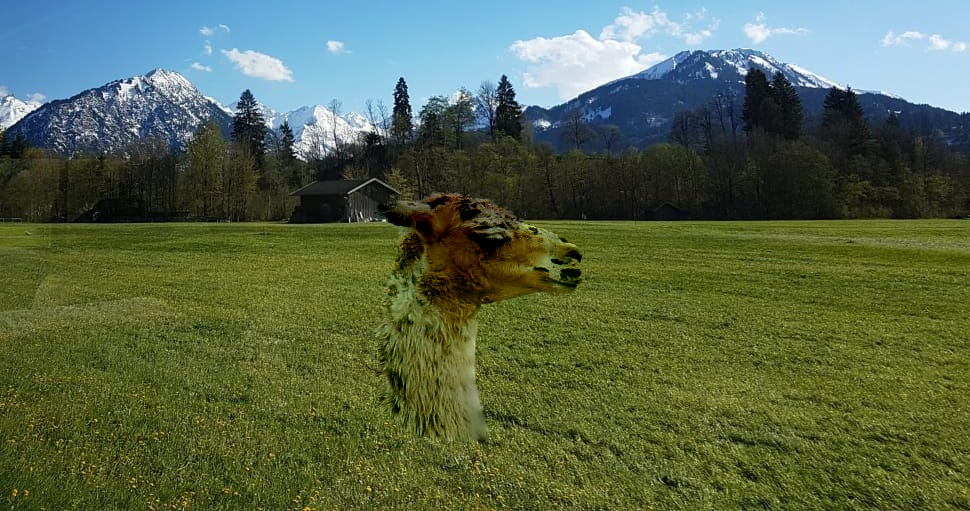
\includegraphics[width=0.3\textwidth]{my_reasults/PS_res/llama_result.png} & 
        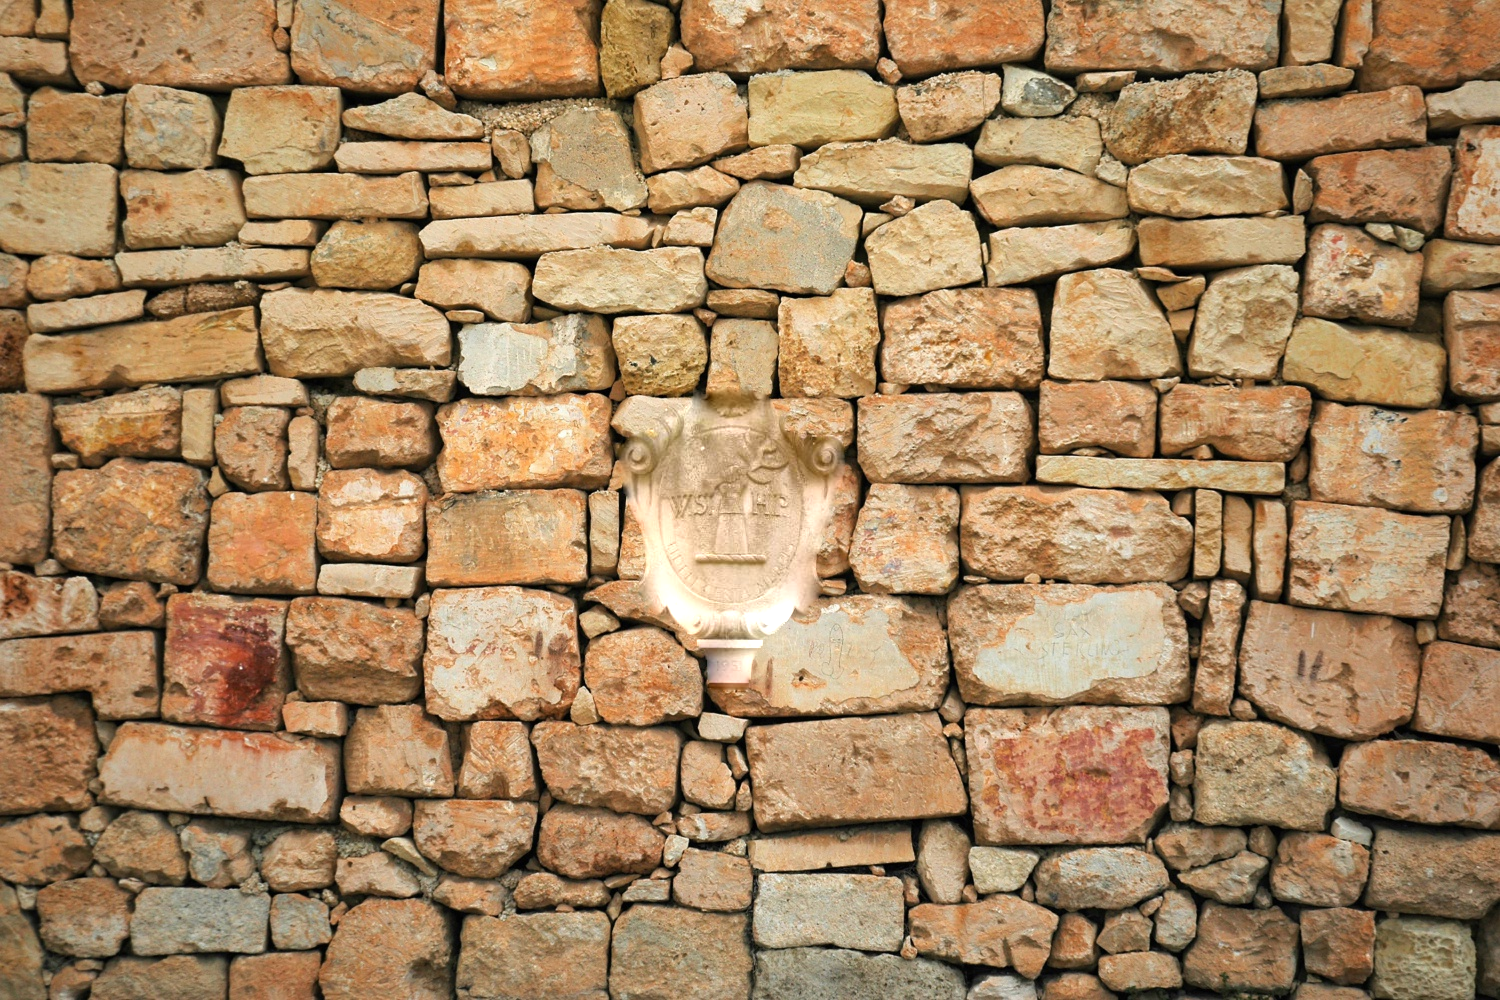
\includegraphics[width=0.3\textwidth]{my_reasults/PS_res/memorial_result.png} \\
        \textbf{Grave} & \textbf{Llama} & \textbf{Memorial} \\
        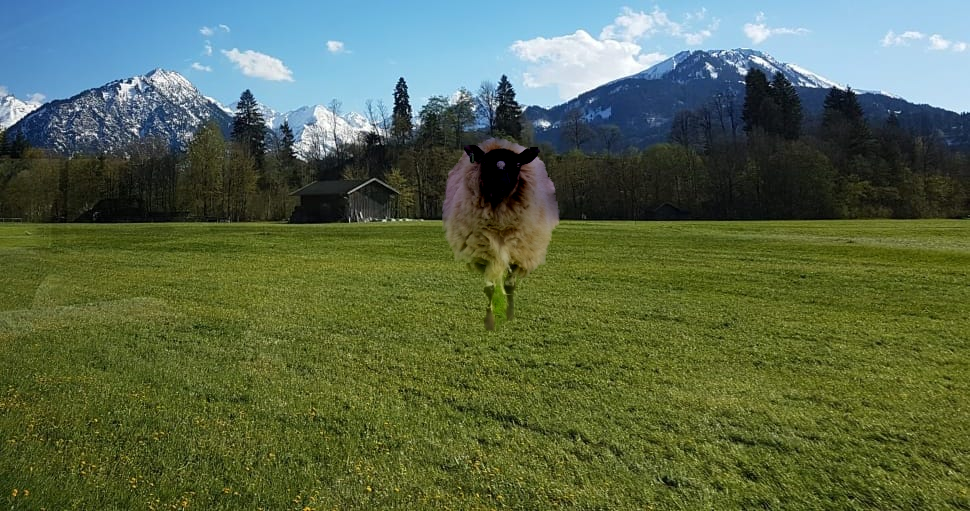
\includegraphics[width=0.3\textwidth]{my_reasults/PS_res/sheep_result.png} & 
        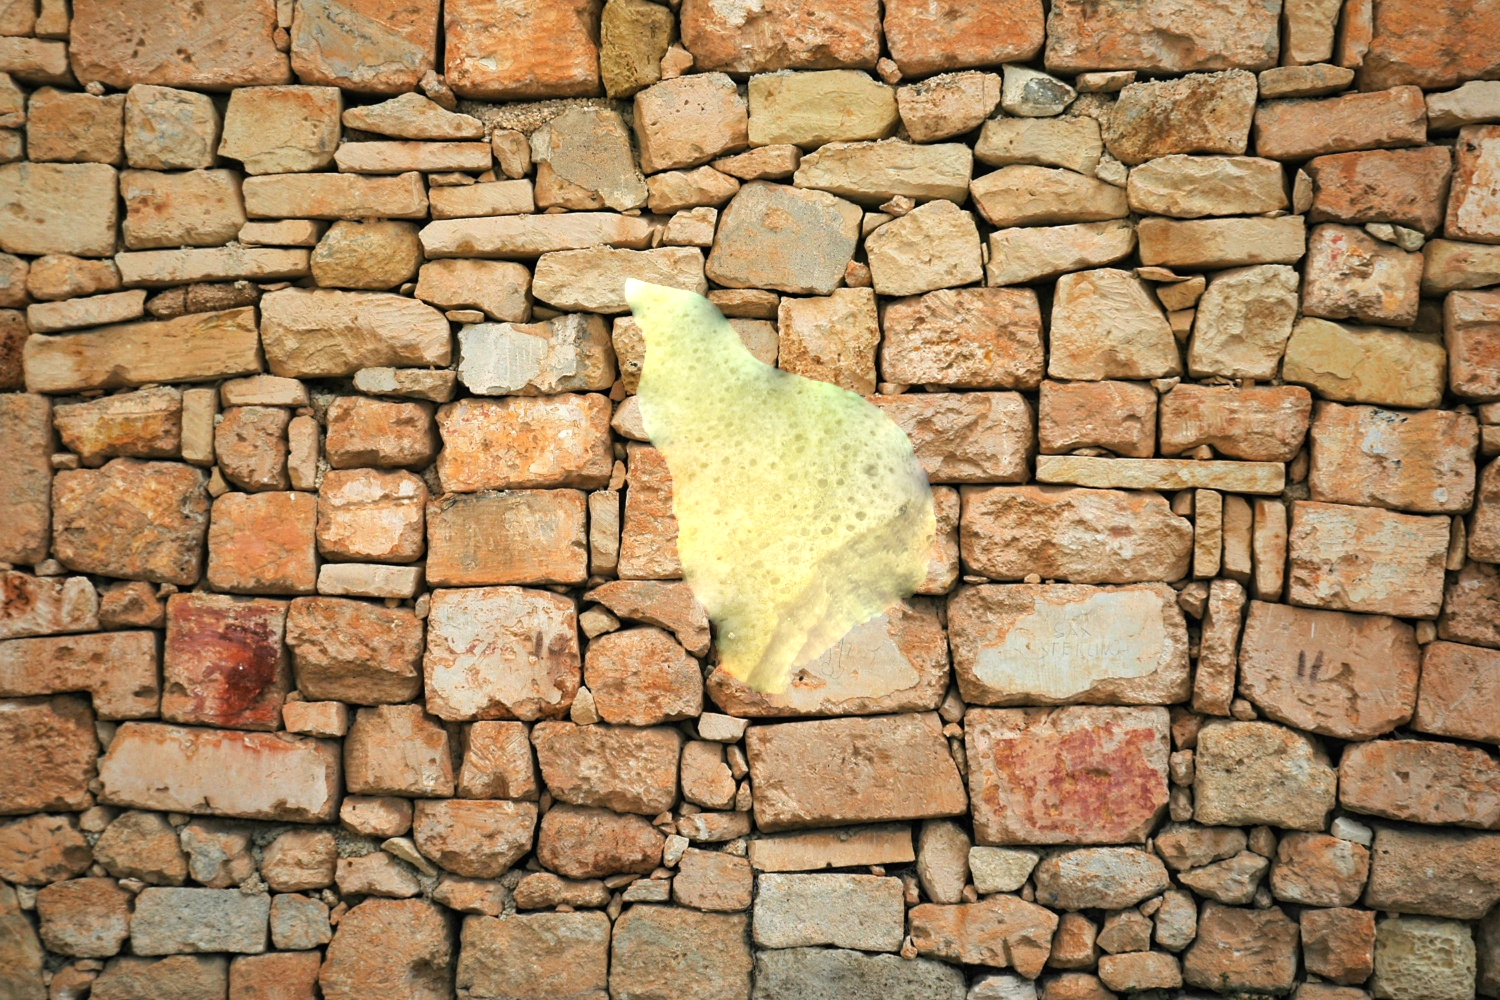
\includegraphics[width=0.3\textwidth]{my_reasults/PS_res/stone_result.png} & 
        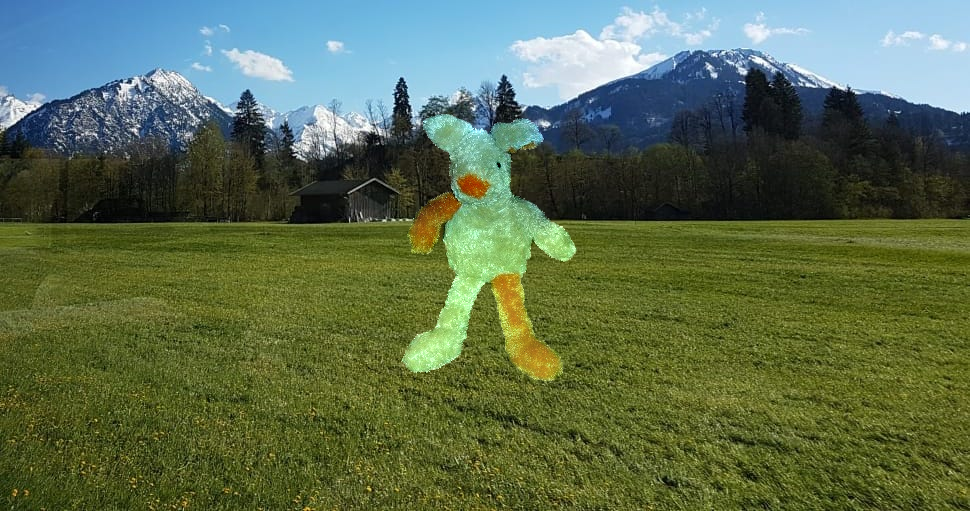
\includegraphics[width=0.3\textwidth]{my_reasults/PS_res/teddy_result.png} \\
        \textbf{Sheep} & \textbf{Stone} & \textbf{Teddy} \\
    \end{tabular}
    \caption{תוצאות Poisson Blending עבור התמונות השונות.}
    \label{fig:ps_results}
\end{figure}

\end{document}
